\chapter{Methodology}\label{methodology}

\section{Requirements}\label{methodology:s:requirements}

\subsection{Current Architecture}\label{methodology:ss:current-architecture}

The current software architecture is still in use as of the date of publication of this body of work. This older architecture consists of an amalgamation of Docker containers, each running a different service. Each Client has its own \gls{vps} wherein these Docker containers are deployed. 

\subsubsection{\gls{vpc}}\label{methodology:sss:vpc}

These \gls{vps} are general-purpose \gls{aws} \gls{ec2} \textit{Instances}. As can be seen on the diagram presented on \Cref{fig:old-arch-overview}, these instances are deployed to the same \gls{vpc}, sharing a private network between them. The Reverse Proxy serves as, as the name implies, as a reverse proxy to enable the use of a single \gls{eip}, a single \gls{eni} by all Clients's servers, since the availability of public IPs is limited to five \gls{eip}.
\begin{figure}[!htbp]
    \centering
    
\includegraphics[width=0.90\textwidth]{img/diagrams/pdf/old-arch-overview.drawio.pdf}
    \caption[AWS VPC Overview]{The AWS VPC used, hosting the old architecture's EC2 \gls{vps}.}
    \label{fig:old-arch-overview}
\end{figure}
    


Each \gls{ec2} instance runs a Docker container for each one of the following services:

\begin{itemize}

\item \textbf{InfluxDB} (Timeseries Database)
\item \textbf{MongoDB} (General use, no-SQL, Document Database)
\item \textbf{Grafana} (Web platform for data visualization, the front end of the \gls{dss})
\item \textbf{Telegraf} (Data collecting service)
\item \textbf{Nginx} (Reverse proxy with \gls{https} capabilities)
\item \textbf{Let's Encrypt} (Automatic \gls{tls} Certificate installer, companion for the Nginx container)
\item \textbf{Web Dev} (Web platform / API for managing Workers' settings)
\item \textbf{Redis} (Message Queue System for queuing Worker's jobs)
\item \textbf{OpenSSH} (\textit{atmoz/sftp}) (\gls{ssh} Server for receiving client data through \gls{sftp})
\item \textbf{Workers} (Container running the Forecast, Simulation and Optimization Python Algorithms as well as the \gls{kpi} Algorithms.)
\item \textbf{Workers} (\textit{Beat}) (Container that periodically \textit{triggers} jobs in the Workers container)

\end{itemize}

\begin{figure}[!htbp]
    \centering
    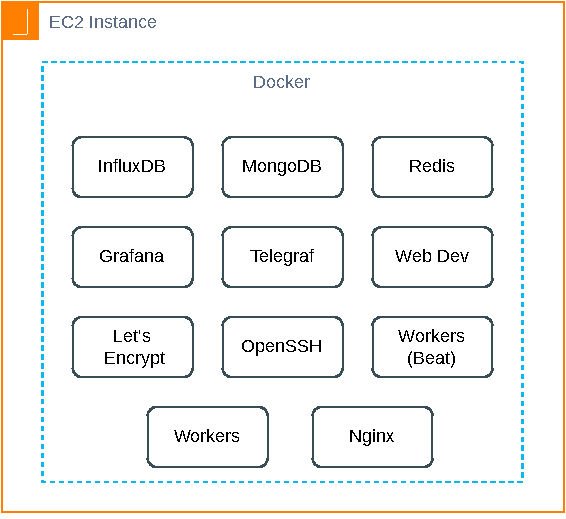
\includegraphics[width=0.75\textwidth]{img/diagrams/pdf/old-arch.drawio.pdf}
    \caption[AWS EC2 VPS Overview]{An AWS EC2 VPS, hosting the old architecture's docker containers}
    \label{fig:old-arch.drawio.pdf}
\end{figure}
    


\subsubsection{Databases}\label{methodology:sss:databases}

There are two types of databases being used by this architecture: A Timeseries Database, in this case \textbf{InfluxDB}, and an additional general-purpose Document Database: \textbf{MongoDB}. Each type of database has a different role, the first one stores the Client's timeseries data such as sensor information, pump orders, predicted tank levels, etc.
The second one, the Document Database, is responsible for storing configuration settings for each worker service (optimization, simulation and forecasting), for storing electrical tariffs data and to store sensor device's configurations.

\subsubsection{Grafana}\label{methodology:sss:grafana}

This web platform allows the visualization of the Timeseries data from the \textbf{InfluxDB} database. This is a freely-available platform that runs on a docker container with little to no modifications necessary. The dashboards are built using the built-in tools and allow for complex and very informative data visualization. This is used in both the new and old architecture, since the new visualization platform is still not operational (not within the scope of this body of work).

\subsubsection{Telegraf}\label{methodology:sss:telegraf}

The \textbf{Telegraf} container is used to gather the files containing the raw sensor data sent from the Client to the \gls{sftp} server. Since this container shares the file upload location folder with the \gls{sftp}, through a convoluted process of storing the filename of the last file uploaded, periodically checking for the next file and file handling \textit{spaghetti} code that spans multiple files and has an enormous codebase that weighs the docker image's file size considerably. 

\subsubsection{\gls{sftp}}\label{methodology:sss:sftp}

The \gls{sftp} service here provides a secure method for the Clients to send files containing the Timeseries data to our servers, where they can be processed and turned into actionable insights by the algorithms running in the Workers container. The Client sends their public key (from a cryptographic key pair) when the project start to authenticate against this \gls{sftp} service and uploads the files to a pre-designated folder. These files are then accessed by the Telegraf container which does the file intake.


\subsubsection{Nginx + Let's Encrypt}\label{methodology:sss:nginxletsencrypt}

These two containers allow secure Internet access from the \gls{ec2} instance into the correct docker container IP address and port. The Client-facing services Grafana and \gls{sftp} which, respectively, provide the web interface for the \gls{dss} and client file input service are inside containers which themselves can change their internal IP inside the Docker environment. To keep the dynamic IPs in check and allow for these services to be accessed from outside the Docker environment the Nginx container keeps track of this dynamic IP and updates its route table accordingly. This allows for any of these two containers to restart, change their IP address and still not break the routing back to the host \gls{ec2} instance, which has an \gls{eni} associated to it exclusively. This \gls{eni} is then connected, exclusively, to a single \gls{eip} to which the Clients connect, like \Cref{fig:old-arch-nginx} implies.

As for the Let's Encrypt container, this container shares a docker volume with the Nginx container and automatically and periodically maintains the \gls{tls} certificate files that the Nginx requires in order to serve the Grafana interface through \gls{https}. 
\begin{figure}[!htbp]
    \centering
    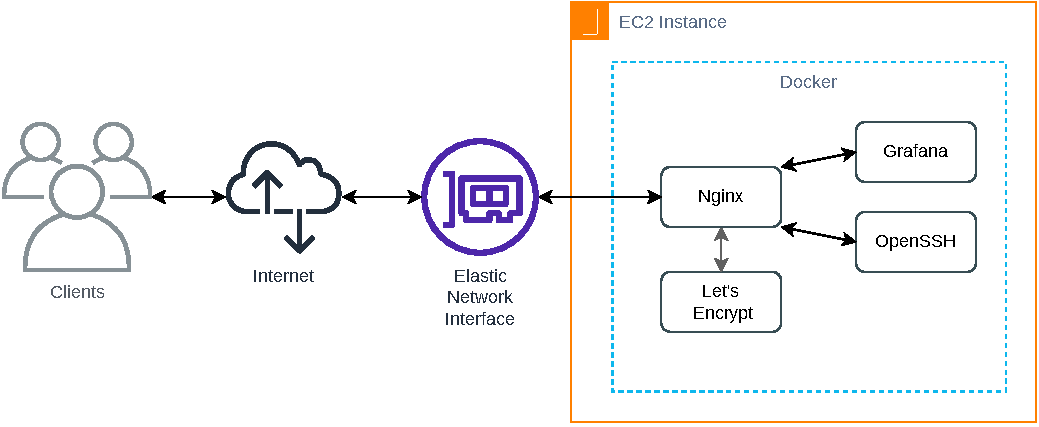
\includegraphics[width=0.90\textwidth]{img/diagrams/pdf/old-arch-nginx.drawio.pdf}
    \caption[Internet access to the Client-facing services]{Internet access to the Client-facing services.}
    \label{fig:old-arch-nginx}
\end{figure}


\subsubsection{Redis}\label{methodology:sss:redis}

We use Redis \parencite{redis_2022} as a message queue backend for Celery \parencite{celery}, enabling other services to send Celery tasks to a queue for asynchronous execution by the Workers.

\subsubsection{Web Dev}\label{methodology:sss:webdev}

Based on Flask \parencite{pallets_2022}, this web application serves an \gls{api} as well as serving a web page that gives developers access to algorithm configurations and the ability to push Celery tasks to the queue. This application connects directly to both databases.

\subsubsection{Workers}\label{methodology:sss:workers}

This is where the \textit{magic} happens. The Workers' container image is built \textit{in-house} by the development team, using a \textit{Python} Docker image as the base image, wherein all the company's algorithms lay. The \textit{forecast}, \textit{optimization} and \textit{performance analysis}/\gls{kpi} algorithms are individually linked in a Celery configuration file, which defines how each algorithm is executed in a Celery task and how that task is called. This container executes a Celery Worker that executes all Celery Tasks in the Celery task queue.

When a task is sent to the task queue, this Celery Worker who polls the task queue, picks the task up and starts executing the task as soon as possible.

There are two Workers images, the first one contains the code for all algorithms and is the one which starts the Celery worker. The other one, which is internally called Celery Beat, executes a Celery instance in \textit{Beat} mode which sends pre-configured Celery tasks to the queue. This is used to run the algorithms periodically in order to process the Client data and generate actionable insights for the Client.

These algorithms require decent amounts of computer resources, namely CPU power and RAM capacity, in order to be able to run effectively. This is a direct contrast to the remaining components of this old architecture, which see minimal Client use and are therefore less resource intensive. In terms of storage, the situation is the opposite since these algorithms use data stored within the other services: the database services.

\begin{figure}[!htbp]
    \centering
    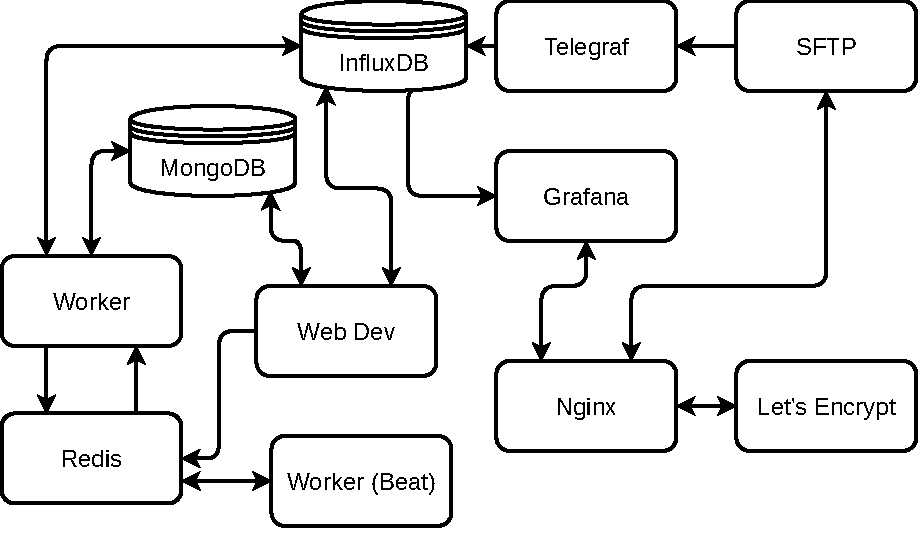
\includegraphics[width=0.90\textwidth]{img/diagrams/pdf/old-arch-connections.drawio.pdf}
    \caption[old-arch-connections listing]{old-arch-connections caption under figure}
    \label{fig:old-arch-connections}
\end{figure}


In \Cref{fig:old-arch-connections} we can see the relations between these containers. Starting on the right side, with the  Let's Encrypt and Nginx containers, these provide outside access to the Grafana and SFTP services inside the respective containers. Data from the InfluxDB database is read by the Grafana service which allows the Client's users and the company's developers to query the database and at the same time generate graphs with such information. Client sensor data is sent to the SFTP server that shares the incoming files with the Telegraf service and allows it to pre-process that sensor data and proceed to the data intake into the InfluxDB database. Then, either through remote access to the Web Dev container or automatically through the Worker Beat service, tasks are sent to the celery queue (using the Redis service) and picked up by the Worker service. This Worker service then accesses the MongoDB Database to load algorithm and device configurations and the required client sensor data from the InfluxDB database before running the tasked algorithm. Data resulting from the execution of the algorithms is then sent to the InfluxDB database, to be read by the Grafana service. There are some connections that are bidirectional, such as the Web Dev to the MongoDB database which is the service used to manipulate the MongoDB database's algorithm and device configurations.

\section{Issues}\label{methodology:s:issues}

\subsection{Resource Sizing}\label{methodology:ss:resource sizing}

\begin{figure}[!htbp]
    \centering
    \fbox{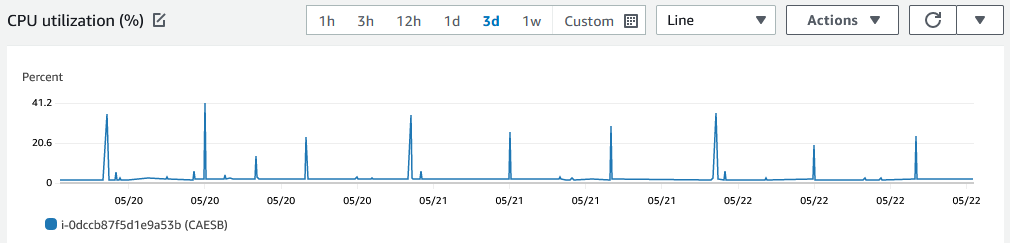
\includegraphics[width=0.95\textwidth]{img/screenshots/caesb-cpu-usage.png}}
    \caption[Client CPU Usage Example]{Client's \gls{ec2} Instance average CPU usage, during a three-day period, in 5 minutes intervals.}
    \label{fig:caesb-cpu-usage}
\end{figure}
    

The contrast between the different services' computational and storage requirements is one of the major issues with the old architecture. Adequate instance sizing is essential to lower infrastructure costs with compute resources. As can be seen in \Cref{fig:caesb-cpu-usage}, the CPU average utilization is usually very low, indicating that the resources allocated to this instance are way overestimated, elevating the infrastructure costs for no reason. However, the peaks in CPU usage that can be observed in this same Figure, which are caused by the periodically-running algorithms, push this CPU usage up to levels that suggest the allocated resources are somewhat adequate for this use-case. And wherein lies one of the major issues: over a 24-hour period, the amount of time spent with very low CPU usage is visibly and significantly superior to the time spent with adequate CPU usage for the instance size. 

The \gls{ec2} instance upon which these services reside can be provisioned and sized to different computational and storage needs. However, this would mean that it would either be adequately sized for the times the workers are dormant and undersized for when the algorithms are running, or oversized for most of the time and only adequately sized while running said algorithms. Unfortunately, resizing an \gls{ec2} instance requires downtime for the whole platform, since it requires the \gls{ec2} instance to be rebooted. Since this would also stop Client access to the \gls{dss} and data intake service, this option cannot be contemplated. After testing a platform implementation with an instance adequately sized for when the workers are dormant, the development team came to the conclusion that the algorithms would either refuse to run or crash when performing resource intensive calculations due to low RAM availability. The decision was then made, to keep the platform running in oversized, and costly, \gls{ec2} instances.

Therefore, one of the goals of this work is to attempt to solve this problem. One of the possible general solutions was to split the resources based on their compute resource requirements. Having the workers on a separate \gls{ec2} instance that would be automatically and periodically provisioned and unprovisioned according to a schedule would allow the remaining services to be placed in a lower cost \gls{ec2} instance, lowering the overall infrastructure costs. However, without altering the existing architecture, this would mean that the alteration would only be the place where the Workers' docker container would be executed. Since the amount of \gls{ec2} instances is directly proportional to the amount of Clients, having two instances would duplicate the computational resources, networks connections and storage space needed to maintain the platform for all Clients. This would exacerbate the problem of limited compute resources available to our \gls{aws} account.

\subsection{Limited Compute Resources}\label{methodology:ss:limited-compute-resources}

One of the issues with the old architecture is that the number of \gls{ec2} instances needed was directly tied to the amount of Clients, since each Client required its own instance to host the platform, generating what is called a Scalability problem. For the company's \gls{aws} account, a limit of thirty-two (32) \gls{vcpu} units (each \gls{vcpu} corresponds to a processing thread in a CPU core) was imposed by Amazon as default, which meant that the sum of \gls{ec2} instance's \gls{vcpu} units could not surpass this value. Each client requires an \gls{ec2} instance of the type \textit{t3a.large} or \textit{t3a.xlarge}, respectively two (2) or four (4) \gls{vcpu} units, depending on the Client's Water Network's size and complexity and contracted services. This would mean that the amount of clients was limited from sixteen (16) clients if they all used the smaller instance or down to eight (8) clients if these Clients required more resources. As can be concluded this is a hard limit on the amount of clients that can be served simultaneously by the company, which is an obvious problem.

\subsection{Individual Codebases}\label{methodology:ss:individual-codebases}

Besides an individual \gls{ec2} instance, each Client also has an individual GitLab \parencite{gitlab_2022} project, which is composed of several, different, Git \parencite{git} code repositories. Each GitLab project contains the following repositories:

\begin{itemize}

    \item \textbf{dbs} (Databases configurations, build files for databases' docker images, deployment scripts)
    \item \textbf{Workers} (Build files for the Workers' docker images)
    \item \textbf{DBconnectors} (Standardized code for database access)
    \item \textbf{forecast\_optimization\_api} (Code and build files for the Web Dev docker image)
    
\end{itemize}

In the \textbf{dbs} repository, we can find build scripts for custom docker images for InfluxDB, Nginx and Telegraf. Also, here reside the scripts that are used to remotely deploy docker containers to the \gls{ec2} instances as well as the \textit{docker-compose} configuration files. The GitLab \gls{cicd} pipeline that deploys the old architecture to the instances also resides here.

As for the \textbf{DBconnectors} repository, database connectors can be found. These allow offloading the code that connects to the databases from the algorithms to a separate module, which can be reused throughout the same GitLab Project and, in theory, keep the query methods consistent for both the \textbf{Workers} and \textbf{Web Dev} codebases.

In the \textbf{Workers} repository, we can find the code for the algorithms used by the platform to perform the forecasting, optimization and KPI calculation as well as the \textbf{DBconnectors} repository linked as a submodule.

In the likeness of the \textbf{Workers} repository, the \textbf{forecast\_optimization\_api} repository also imports the \textbf{DBconnectors} repository as a submodule. This \textbf{forecast\_optimization\_api} repository is where the \textit{Web Dev} container build code is situated. 

Astute readers will notice that, as shown both above and on \Cref{fig:old-arch-connections}, that there are multiple services performing read and write operations to the InfluxDB database. Although concurrency is not a major problem, having different schemas and tag names for InfluxDB queries in different services has historically led to multiple timeseries data not being detected when querying the database when the service querying it was not the same that placed the data in the database. This is due to mismanagement of repositories and git submodules, and requires additional care, planning and communication from the developer team's side. Here, having a specific service to perform pre-prepared queries, with very detailed database schemas, to which all other services would connect to query/write to the database would solve this problem.\textcolor{red}{(citation needed)}


\subsection{Deployment}\label{methodology:ss:deployment}

When deploying new functionality or code fixes to Client's servers that use the old architecture, this process can quickly become a multi-hour endeavor. Despite being a somewhat modular architecture, given that each service has its own docker container, they are dependent on each other when initializing the containers. On some deployment procedures, namely when changing code in the Workers container, it requires updating the Workers' docker image, running GitLab's \gls{cicd} pipelines for this deployment of the Workers' docker image and then tag a completely different repository —  \textbf{dbs} — inside the same Client's GitLab project so that it triggers another \gls{cicd} pipeline which replaces all the containers within the Client's \gls{ec2} instance with the \textit{latest} version of each service's container image. Although the last step, which replaces the containers is performed rather quickly and the apparent downtime for the Client is minimal, the amount of time for the image building in the \gls{cicd} process is cumbersome, reaching a combined time of 20 to 30 minutes on average. This chaotic and time-consuming process leads to lack of motivation from the development team to introduce new features regularly. This leads to lower Deployment Frequency, increased Lead Time for Change and Time to Restore Service (when a deployment or unexpected bug occurs). Additionally, the complexity and tight-coupling of services leads to increase Change Failure Rate. 




